\documentclass[12pt]{article}

\usepackage[utf8]{inputenc}
\usepackage{comment}
\usepackage{hyperref}
\usepackage{listings}
\usepackage{graphicx}
\usepackage{titlesec}
\usepackage{hyperref}
\usepackage{blindtext}
\usepackage{enumitem}
\usepackage{fancyhdr}
\usepackage{afterpage}
\usepackage{biblatex}


\newcommand{\noopsort}[1]{} \newcommand{\printfirst}[2]{#1}
  \newcommand{\singleletter}[1]{#1} \newcommand{\switchargs}[2]{#2#1}

\pagestyle{fancy}
\fancyhf{}
\lhead{\rightmark}
\rhead{Page \thepage}
%\cfoot{\thepage}

\newcommand\blankpage{%
    \null
    \thispagestyle{empty}%
    \addtocounter{page}{-1}%
    \newpage}

\titleclass{\subsubsubsection}{straight}[\subsection]

\newcounter{subsubsubsection}[subsubsection]
\renewcommand\thesubsubsubsection{\thesubsubsection.\arabic{subsubsubsection}}
\renewcommand\theparagraph{\thesubsubsubsection.\arabic{paragraph}} % optional; useful if paragraphs are to be numbered

\titleformat{\subsubsubsection}
  {\normalfont\normalsize\bfseries}{\thesubsubsubsection}{1em}{}
\titlespacing*{\subsubsubsection}
{0pt}{3.25ex plus 1ex minus .2ex}{1.5ex plus .2ex}

\makeatletter
\renewcommand\paragraph{\@startsection{paragraph}{5}{\z@}%
  {3.25ex \@plus1ex \@minus.2ex}%
  {-1em}%
  {\normalfont\normalsize\bfseries}}
\renewcommand\subparagraph{\@startsection{subparagraph}{6}{\parindent}%
  {3.25ex \@plus1ex \@minus .2ex}%
  {-1em}%
  {\normalfont\normalsize\bfseries}}
\def\toclevel@subsubsubsection{4}
\def\toclevel@paragraph{5}
\def\toclevel@paragraph{6}
\def\l@subsubsubsection{\@dottedtocline{4}{7em}{4em}}
\def\l@paragraph{\@dottedtocline{5}{10em}{5em}}
\def\l@subparagraph{\@dottedtocline{6}{14em}{6em}}
\makeatother

\setcounter{secnumdepth}{4}
\setcounter{tocdepth}{4}

 \hypersetup{
    colorlinks=true,
    linkcolor=black,
    filecolor=magenta,      
    urlcolor=cyan,
}

\urlstyle{same}

\title{\bf{Intelligence Transportation System}}
\author{
  Dr.Emad Nabil\thanks{Thank you for help us to make this project done}\\
  \texttt{Doctor in cairo university, egypt}
  \and
  Omar alkubati\\
  20140377\\
  \texttt{omer.alqubati@gmail.com}
  \and
  Mahmoud Mosaad\\
  20140256\\
  \texttt{mahmoudmosaad50@gmail.com}
  \and
  Ziad Aamer\\
  20140341\\
  \texttt{ziadaamer9@gmail.com}
  \and
  Hameed\\
  20140375\\
  \texttt{hameed203083@gmail.com}
  \and
  Aseel\\
  20140367\\
  \texttt{asseel7723@gmail.com}
}
\date{\today }

\begin{document}

\begin{titlepage}
\clearpage\maketitle
\thispagestyle{empty}
\end{titlepage}

\blankpage
%\href{https://github.com/mahmoud-mosaad/transportation-system}{github-fork}
\tableofcontents
\newpage

\section{\sc Project Idea}
Our project idea is to solve the Travelling Salesman problem, this problem appears in Companies that have transportation system and want to minimize the cost of delivering the orders, and this is done by providing the correct order in which salesmans should deliver orders.

\section{\sc Problem Significance}

\subsection{ Problem Definition }
The traveling salesman problem is a common NP hard problem and consists of a salesman and a set of cities. The salesman has to visit each one of the cities starting from a certain one (e.g. the hometown) and returning to the same city. The challenge of the problem is that the traveling salesman wants to minimize the total length of the trip.
\begin{center}
	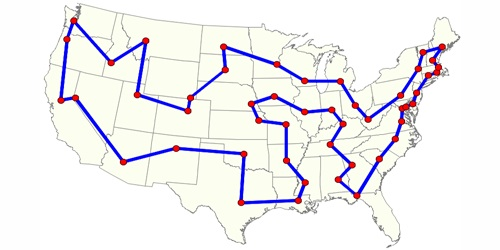
\includegraphics[width=15cm,height=7cm]{./assets/example/tsp.png}\\
\end{center}

\subsection{ The Problem variants }

\subsubsection{ Symmetric (STSP) }
The TSP is symmetric if, for every pair of cities i and j, the distance from i to j is the same as the one from j to i.

\subsubsection{ Asymmetric (ATSP) }
The TSP is asymmetric if, the distance for going from a point to another may be different of the returning distance.

\subsubsection{ The online TSP }
The number of requests n is not known to the online server. Requests are revealed to the online server at their release dates.

\subsubsection{ The price collecting TSP }
In the TSP, the salesman has to visit a set of cities while minimizing the length of the overall tour. In the PCTSP, each city has a given weight and penalty, and the goal is to collect a given quota of the weights of the cities while minimizing the length of the tour plus the penalties of the cities not in the tour.

\subsubsection{ Bus, truck, vehicle routing }
Asks "What is the optimal set of routes for a fleet of vehicles to traverse in order to deliver to a given set of customers?". It generalizes the well-known travelling salesman problem (TSP).

\subsubsection{ Edge/arc and node routing with capacities }
The CARP aims to find a set of vehicle trips with minimum cost, such that each trip starts and ends at a depot node v0 2 V, each required edge.is serviced by a single trip, and the total demand for any vehicle does not exceed a capacity Q.

\subsection{ Motivation }
Assume that you are the driver of a delivery vehicle with a certain set of stops that need to be made each day. How would you determine the order in which to make the stops? If you are interested solely in distance, you could create a graph of the transportation network and weight each edge as the distance of the roadway it represents, allowing a solution to the Traveling Salesman Problem (TSP) to determine the shortest route.

\subsection{ Problem Solution }
Travel Salesman Problem has more than one approach to solve it.\\
e.g:  Exact Approach, Greedy Approach, Heuristic Approach and Genetic Algorithm Approach.

\subsubsection{ Exact Approach }
The solution is optimal but very slow.

\subsubsubsection{  Brute Force }
naive algorithm that generate all possible paths choose the minimum cost path but we will not use it because it has a very high Complexity O(n!) .
\begin{center}
	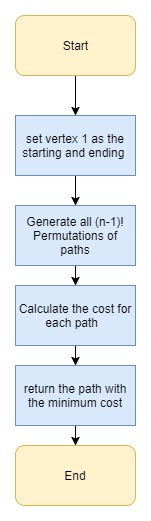
\includegraphics[width=6cm,height=14cm]{./assets/flowchart/brute-force.png}\\
\end{center}

\subsubsubsection{  Dynamic Programming (Held Karp) }
Every sub-path of a path of minimum distance is itself of minimum distance. we will use this algorithm in exact approach as its complexity is O($2^n  n^2$).
\begin{center}
	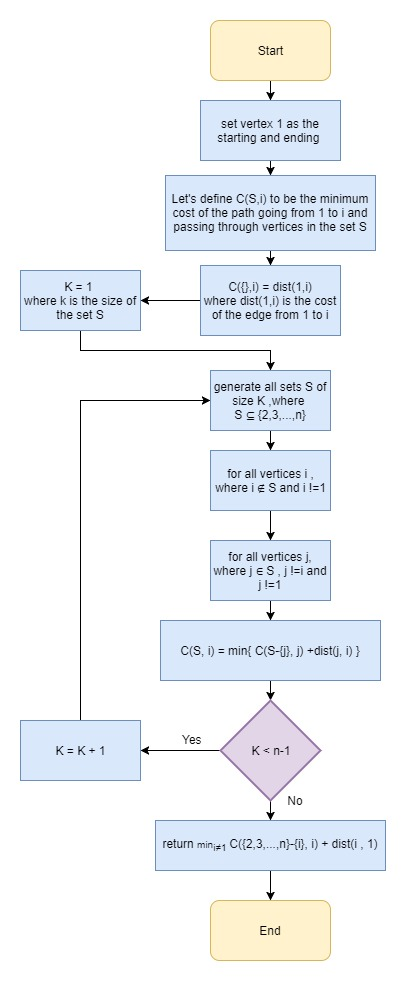
\includegraphics[width=10cm,height=18cm]{./assets/flowchart/held-karp.png}\\
\end{center}

Assuming we run the algorithm on a $10^10$ instructions per seconds processor.
\begin{center}
	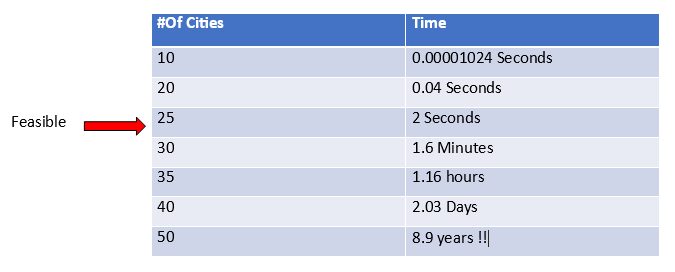
\includegraphics[width=15cm,height=7cm]{./assets/example/db-time.png}\\
\end{center}

\subsubsection{ Heuristic Approach }

\begin{itemize}
\item \bf{Approximation}: 
Solving the TSP optimally takes to long, instead uses approximation algorithms, or heuristics and can get good solutions but may not optimal.
\item \bf{Tour Construction}:
Tour construction algorithms have one thing in commmon,
they stop when a solution is found and never
tries to improve it.
\item \bf{Tour Improvement}:
Once a tour has been generated by some tour construction
heuristic, we might wish to improve that solution.
There are several ways to do this, but the most
common ones are the 2-opt or k-opt local searches.
Their performances are somewhat linked to the construction
heuristic used.
\end{itemize}
\newpage
\subsubsubsection{ Nearest Neighbor Algorithm (Construction)}
An algorithm that choose the best choice that rechable at current state.
Complexity: O(n log(n))
\begin{center}
	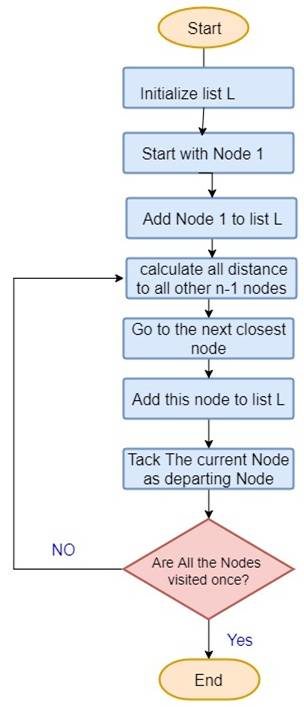
\includegraphics[width=10cm,height=17cm]{./assets/flowchart/greedy.png}\\
\end{center}

\subsubsubsection{ Cheapest Link (Construction)}
\begin{center}
	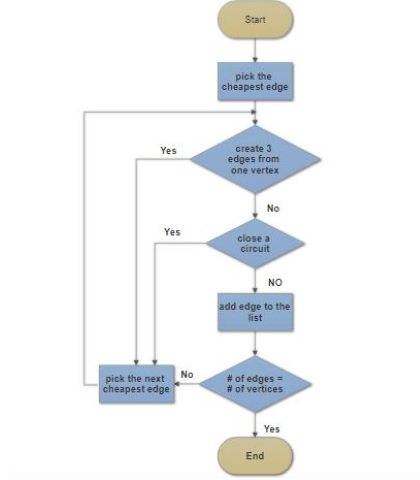
\includegraphics[width=11cm,height=14cm]{./assets/flowchart/cheapest.png}\\
\end{center}

\newpage
\subsubsubsection{ Depth First Tree Tour (Construction)}
This algorithm (DFTT) based on minimum spanning tree (MST) or kruskal's algorithm, the length is exactly twice of the MST's weight, MST weight is not more than length of optimal tour, skipping visited nodes along the DFTT and apply Triangular Inequality, tour length at most twice of optimal length.\\
This flowchart explain all the process.\\
\begin{center}
	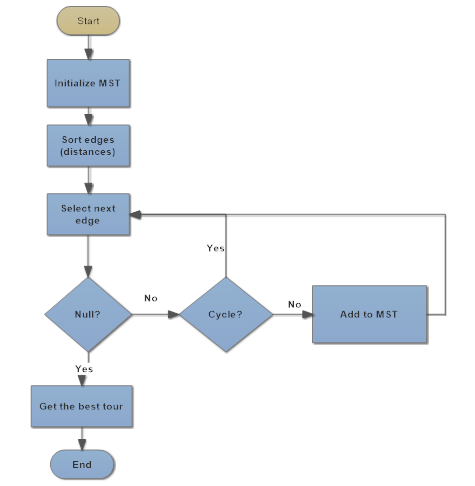
\includegraphics[width=12cm,height=13cm]{./assets/flowchart/dftt.png}\\
\end{center}
\newpage
Graph Example : \\
\begin{center}
	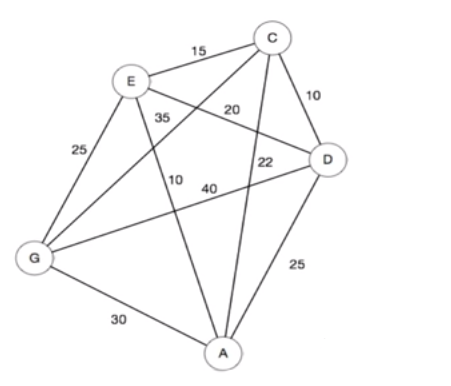
\includegraphics[width=9cm,height=8cm]{./assets/example/graph-dftt-1.png}\\
\end{center}
First get the MST of the graph like in the figure (in red).\\
\begin{center}
	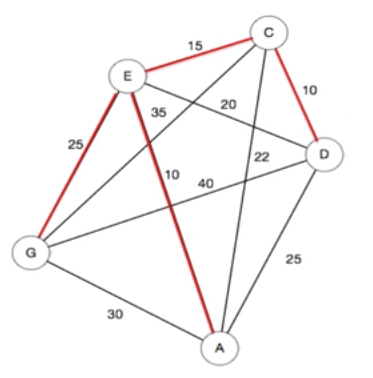
\includegraphics[width=9cm,height=8cm]{./assets/example/graph-dftt-2.png}\\
\end{center}
Traverse the graph along MST edges and double the edges (in blue).\\
\begin{center}
	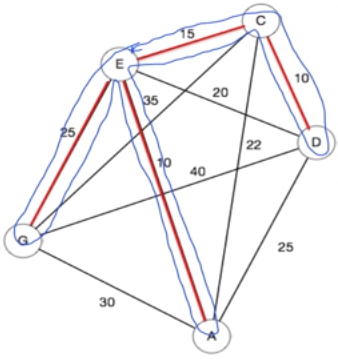
\includegraphics[width=9cm,height=8cm]{./assets/example/graph-dftt-3.png}\\
\end{center}
Last thing is to apply triangular inequality to get the best tour (in green).\\
\begin{center}
	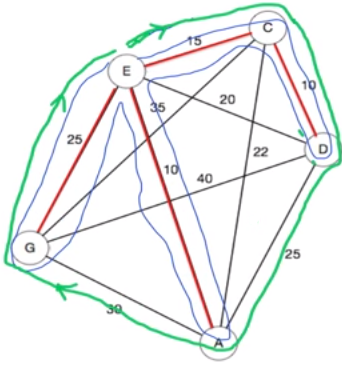
\includegraphics[width=9cm,height=8cm]{./assets/example/graph-dftt-4.png}\\
\end{center}

\subsubsubsection{ 2-opt (Improvement)}
The 2-opt algorithm basically removes two cross over edges
from the tour, and reconnects the two paths created.
There is only one way to reconnect the two paths so that we still
have a valid tour. We do this only if the
new tour will be shorter. Continue removing and reconnecting
the tour until no 2-opt improvements can
be found. The tour is now 2-optimal. this figure explain cross over 2-opt can solve it.
\begin{center}
	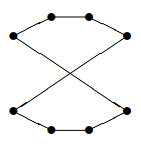
\includegraphics[width=2cm,height=2cm]{./assets/example/graph-2opt-1.png}
\end{center}
This flowchart explain all the process.
\begin{center}
	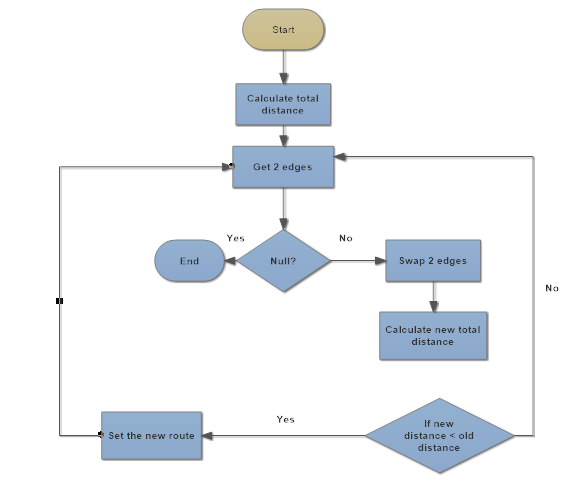
\includegraphics[width=13cm,height=12cm]{./assets/flowchart/2-opt.png}
\end{center}
Look for an improvement obtained by deleting two edges and adding two edges.
\begin{center}
	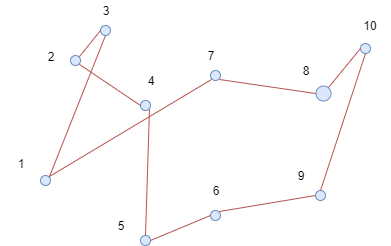
\includegraphics[width=7cm,height=5cm]{./assets/example/2-opt-1.png}
\end{center}
Deleting arcs (4,7) and (5, 1) flips the subpath from node 7 to node 5. 
\begin{center}
	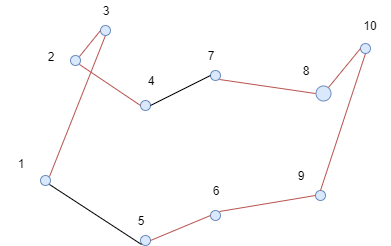
\includegraphics[width=7cm,height=5cm]{./assets/example/2-opt-2.png}
\end{center}
Deleting arcs (1,3) and (2, 4) flips the subpath from 3 to 2. 
\begin{center}
	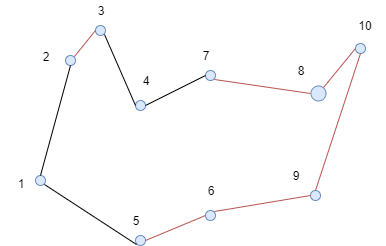
\includegraphics[width=7cm,height=5cm]{./assets/example/2-opt-3.png}
\end{center}
Deleting arcs (7,8) and (10, 9) flips the subpath from 8 to 10. 
\begin{center}
	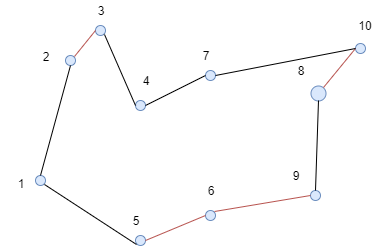
\includegraphics[width=7cm,height=5cm]{./assets/example/2-opt-4.png}
\end{center}

\subsubsubsection{Christofides algorithm (Construction)}
Solutions is guranteed to be within a factor of 3/2 of the optimal solution O($n^3$). The best approximation ratio that has been proven for TSP but it has the constrain that the edges must and obey the triangle inequality. It provides a very good heuristic solutions, but unfortunately it is  impractical because of the constraints it has.

\subsubsection{ Meta Heuristic Approach }
same as Heuristic, but Meta-Heuristic is problem independent and can be applied to a wide range of problems.  

\subsubsubsection{ Genetic Algorithm }
Fitness function:  $$F_{i} = 1 / \sum_{i=1}^{n} Distance(G_{i},G_{i+1})$$
Complexity: O($n^3$).
\begin{center}
	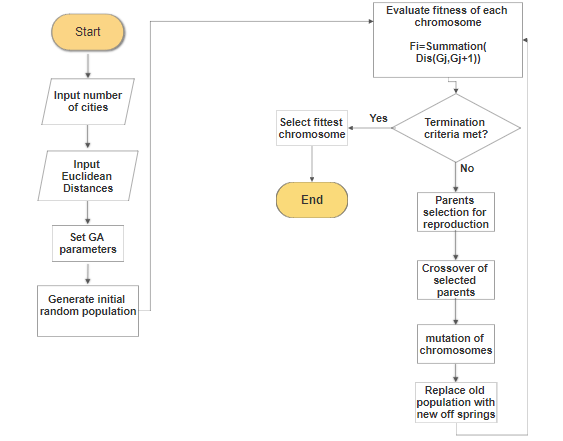
\includegraphics[width=17cm,height=13cm]{./assets/flowchart/ga.png}\\
\end{center}

\subsection{ TSP Solver Modules }
\begin{itemize}
	\item Clustering module.
	\item Route creation module.
\end{itemize}

\subsubsection{Clustering module}
\begin{itemize}
	\item Automation, e.g: K-Means.
	\item Clustering by region.
	\item Manual.
\end{itemize}

\subsubsection{Route creation module}
  If number of cities $>=$ 21 then 
  	Run Exact Algorithm to get best route\\
  Else
        Run all heuristic and meta heuristic 
        algorithms and return the best route resulted
         from all algorithms

\section{\sc System Analysis and Design}

\subsection{ System Architecture }
\begin{center}
	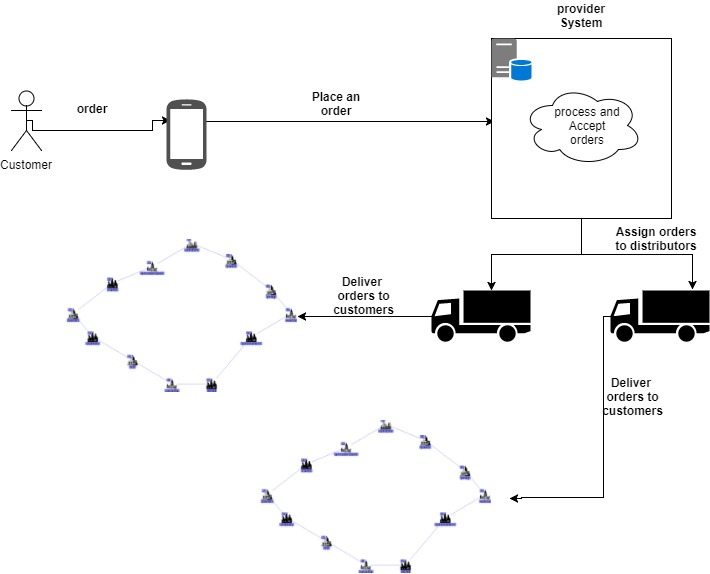
\includegraphics[width=16cm,height=13cm]{./assets/systemarchitecture/system-architecture.png}\\
\end{center}
\newpage

\subsection{ Stakeholders }
A stakeholder can be internal or external. 

\subsubsection{  Customer }
Are External-Operational stakeholders, who make the orders and this stakeholders will interact with the system via Android application.

\subsubsection{  Admin }
Is Internal-Operational stakeholder, who receives the orders and distributes them to the distributors according to the address of the customers, this stakeholder will interact with the system via web application.

\subsubsection{  Salesman }
Is Internal-Operational stakeholder, receives the orders that they should deliver and ask the system to get the optimal route to follow, this stakeholders will interact with the system via Android application.
\newpage

\subsection{ Functional Requirements }

\subsubsection{ Customer }
\begin{itemize}
	\item Order any Product including quantity and location.
	\item Cancel order before distributor takes it.
	\item Update orders in cart.
\end{itemize}

\subsubsection{ Admin }
\begin{itemize}
	\item Reject or accept an order.
	\item Run TSP solver.
	\item Add salesman.
\end{itemize}

\subsubsection{ Salesman }
\begin{itemize}
	\item View requests.
	\item View path.
	\item Confirm request delivery.
	\item Check availablility.
\end{itemize}
\newpage

\subsection{ Non-Functional Requirements }

\subsubsection{ Security }
\begin{itemize}
	\item The System has a form of protection by applying authentication and authorization, so any unauthorized access to the system is denied.
	\item Avoid SQL injection.
	\item Avoid XSS.
	\item Avoid rainbow tables.
\end{itemize}

\subsubsection{ Performance }
\begin{itemize}
	\item Login must be completed in less than 3 seconds.
	\item Peak load 200 user every hour.
	\item Admin assign orders to salesman in less than 10 seconds.
\end{itemize}

\subsubsection{ Reliability }
\begin{itemize}
	\item The system has to be 100\% reliable.
\end{itemize}

\subsubsection{ Availability }
\begin{itemize}
	\item The system will be available 24/7 and making backups.
\end{itemize}

\subsubsection{ Usability }
\begin{itemize}
	\item The customer can easily order any products with any quantities with easy UX.
\end{itemize}

\subsection{ Use Case Diagram }
\begin{center}
	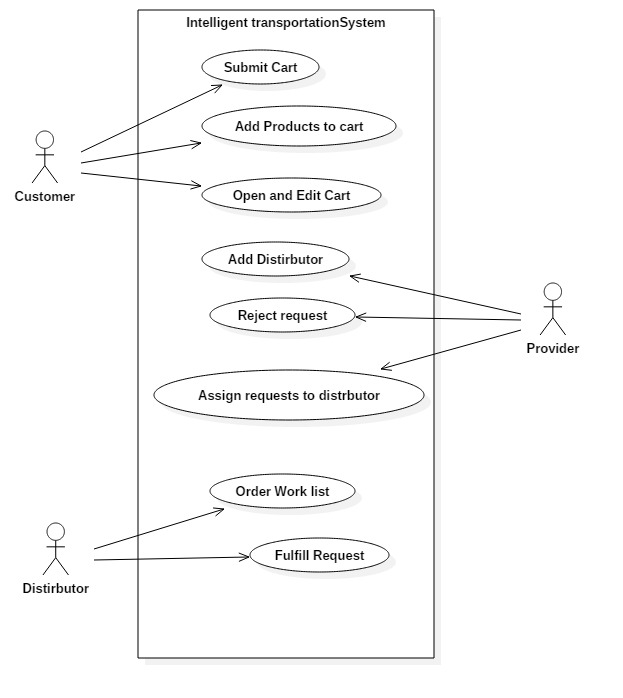
\includegraphics[width=17cm,height=15cm]{./assets/usecase/use-case-diagram.png}\\
\end{center}

\subsection{ Use Case Tables }

\subsubsection{ Customer }
\begin{center}
	\includegraphics[width=17cm,height=15cm]{./assets/usecasetable/customer-1.png}\\
	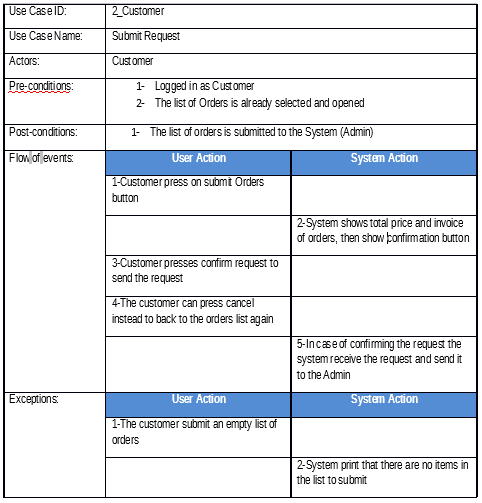
\includegraphics[width=17cm,height=15cm]{./assets/usecasetable/customer-2.png}\\
	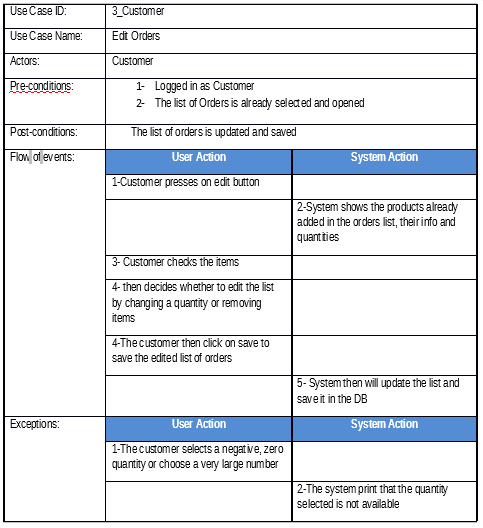
\includegraphics[width=17cm,height=15cm]{./assets/usecasetable/customer-3.png}\\
\end{center}

\subsubsection{ Salesman }
\begin{center}
	\includegraphics[width=17cm,height=15cm]{./assets/usecasetable/distributer-1.png}\\
	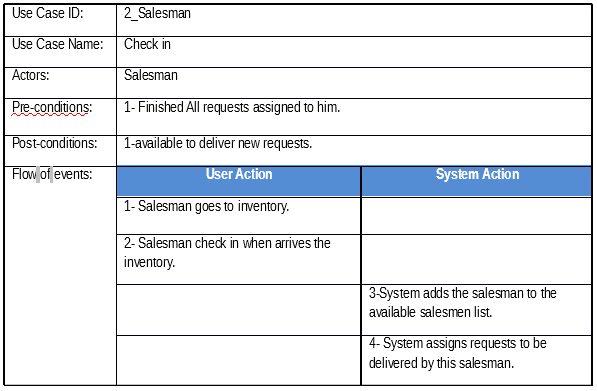
\includegraphics[width=17cm,height=15cm]{./assets/usecasetable/distributer-2.png}\\
\end{center}

\subsubsection{ Admin }
\begin{center}
	\includegraphics[width=17cm,height=15cm]{./assets/usecasetable/provider-1.png}\\
	\includegraphics[width=17cm,height=15cm]{./assets/usecasetable/provider-2.png}\\
\end{center}

\subsection{ Sequence Diagram }

\subsubsection{ Add Order }
\begin{center}
	\includegraphics[width=17cm,height=13cm]{./assets/sequencediagram/addorder.png}\\
\end{center}

\subsubsection{ Edit orders }
\begin{center}
	\includegraphics[width=17cm,height=13cm]{./assets/sequencediagram/editorders.png}\\
\end{center}

\subsubsection{ Reject Requests }
\begin{center}
	\includegraphics[width=17cm,height=13cm]{./assets/sequencediagram/rejectrequests.png}\\
\end{center}

\subsubsection{ Deliver Order }
\begin{center}
	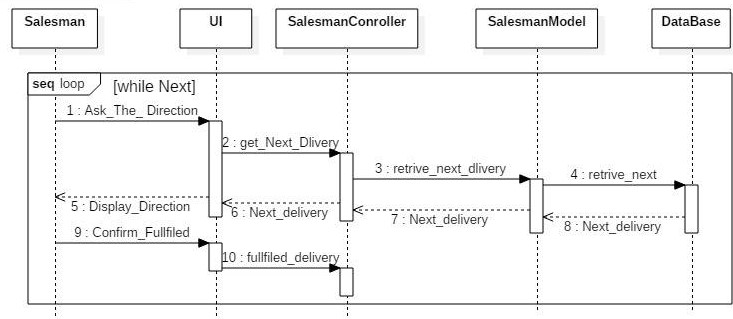
\includegraphics[width=17cm,height=13cm]{./assets/sequencediagram/deliverorder.png}\\
\end{center}

\subsubsection{ Run TSP Solver }
\begin{center}
	\includegraphics[width=17cm,height=13cm]{./assets/sequencediagram/runtspsolver.png}\\
\end{center}

\subsubsection{ Check In Availability }
\begin{center}
	\includegraphics[width=17cm,height=13cm]{./assets/sequencediagram/checkin.png}\\
\end{center}
\newpage

\subsection{ Class Diagram }

\begin{center}
    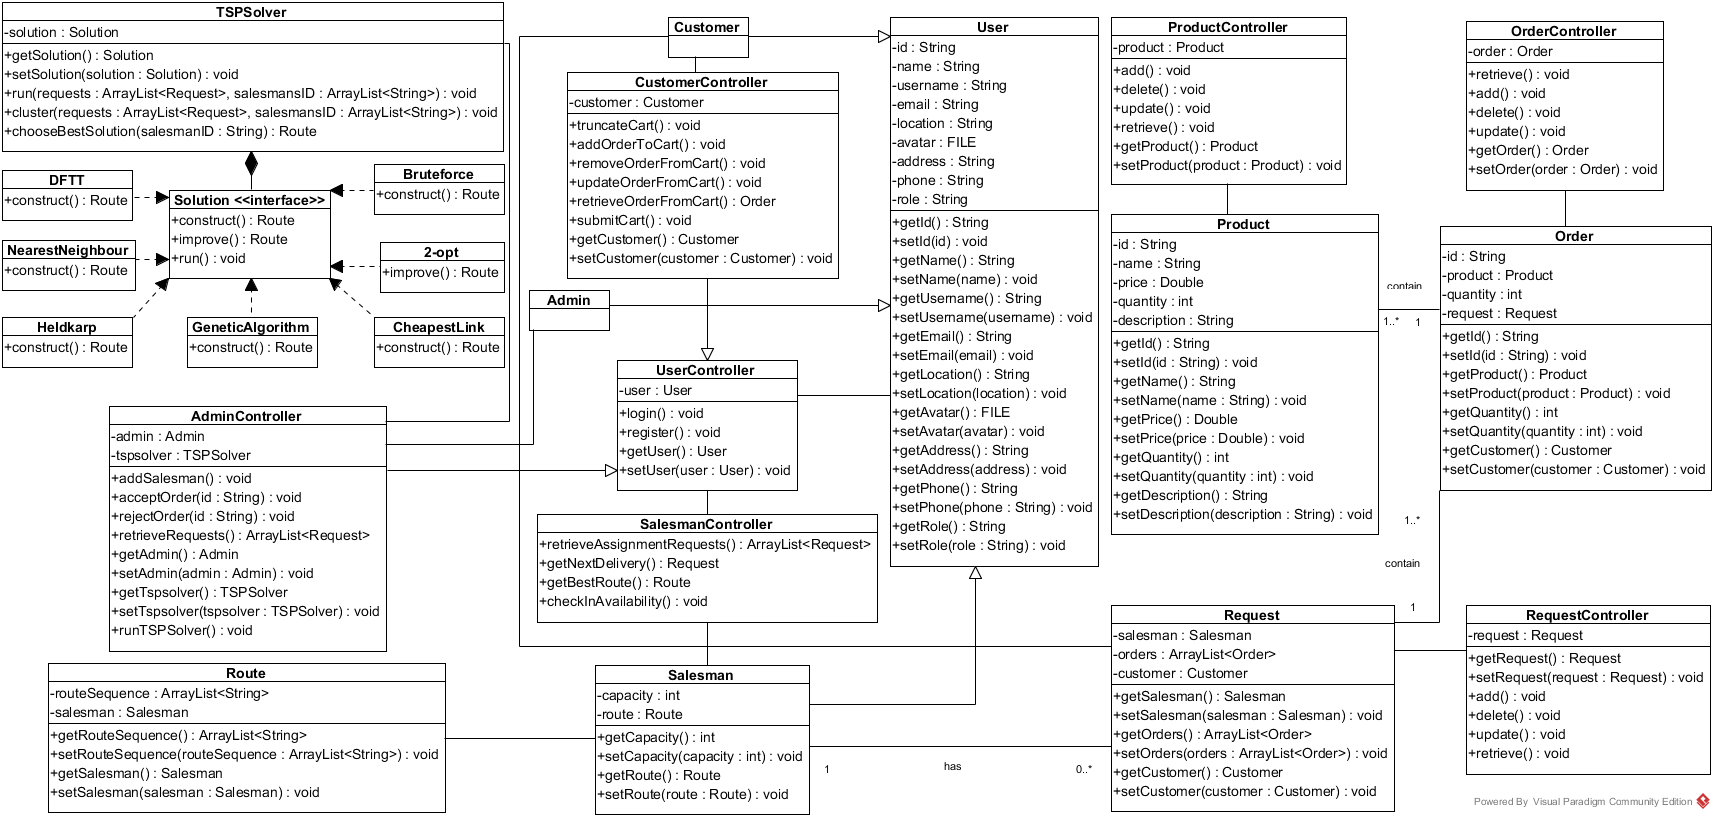
\includegraphics[width=17cm,height=11cm]{./assets/class-diagram.png}
\end{center}
\newpage

\subsection{ ERD (Entity Relationship Diagram) }

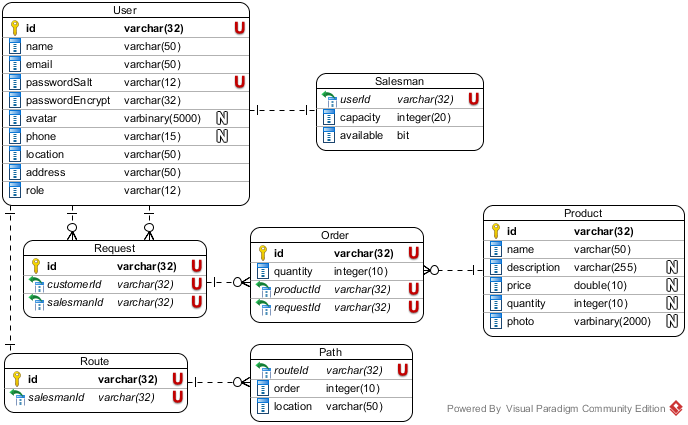
\includegraphics[width=17cm,height=10.5cm]{./assets/erd.png}


\subsection{ Prototype }

\subsubsection{ Salesman }
\includegraphics[width=16cm,height=10cm]{./assets/prototype/distributer-1.png}\\

\subsubsection{ Admin }
\includegraphics[width=16.5cm,height=7cm]{./assets/prototype/provider-1.png}\\
\includegraphics[width=16.5cm,height=10cm]{./assets/prototype/provider-2.png}\\

\subsubsection{ Customer }
\includegraphics[width=16cm,height=10cm]{./assets/prototype/customer-1.png}\\

\subsection{ Gantt chart }

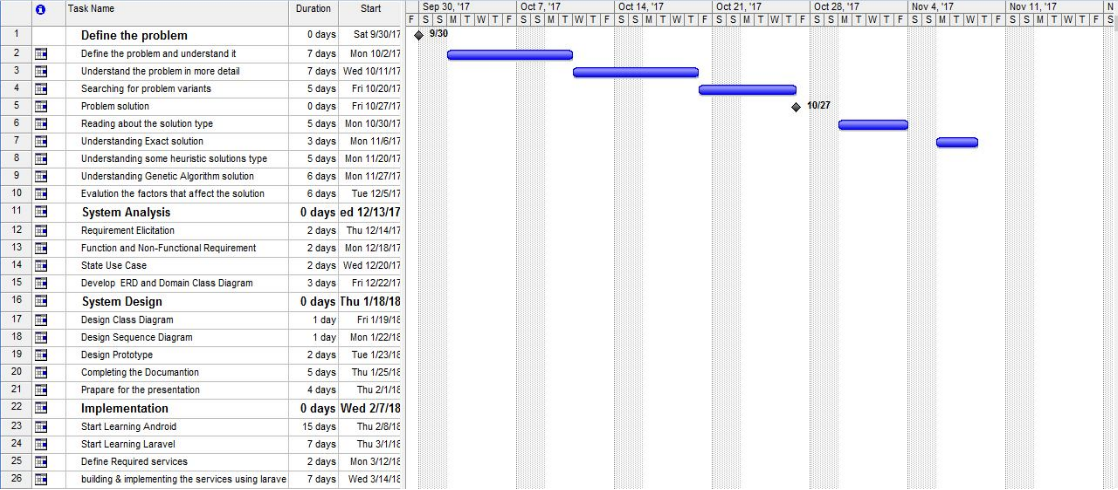
\includegraphics[width=17cm,height=8.5cm]{./assets/ganttchart/gantt-1.png}\\
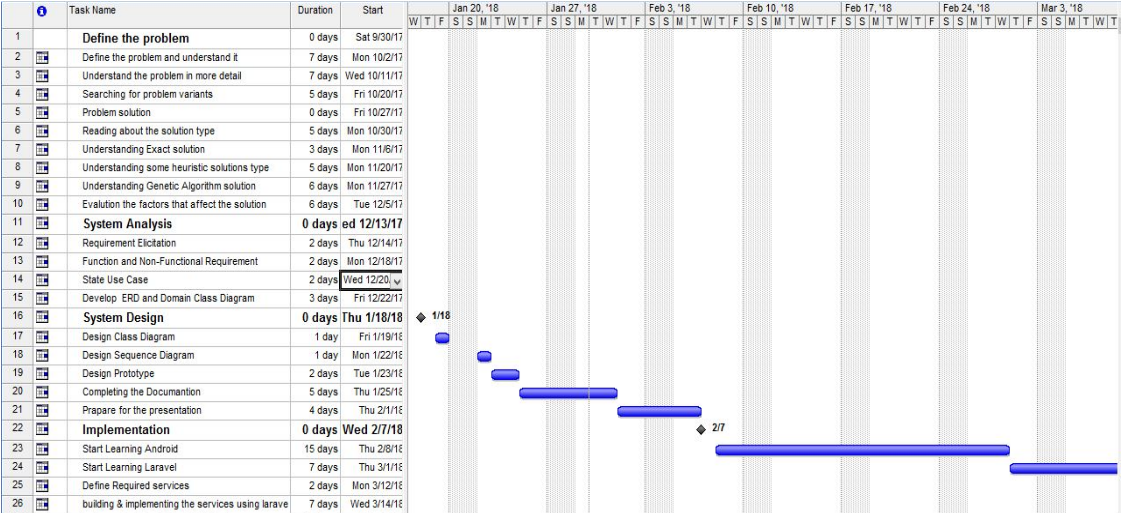
\includegraphics[width=17cm,height=8.5cm]{./assets/ganttchart/gantt-2.png}\\
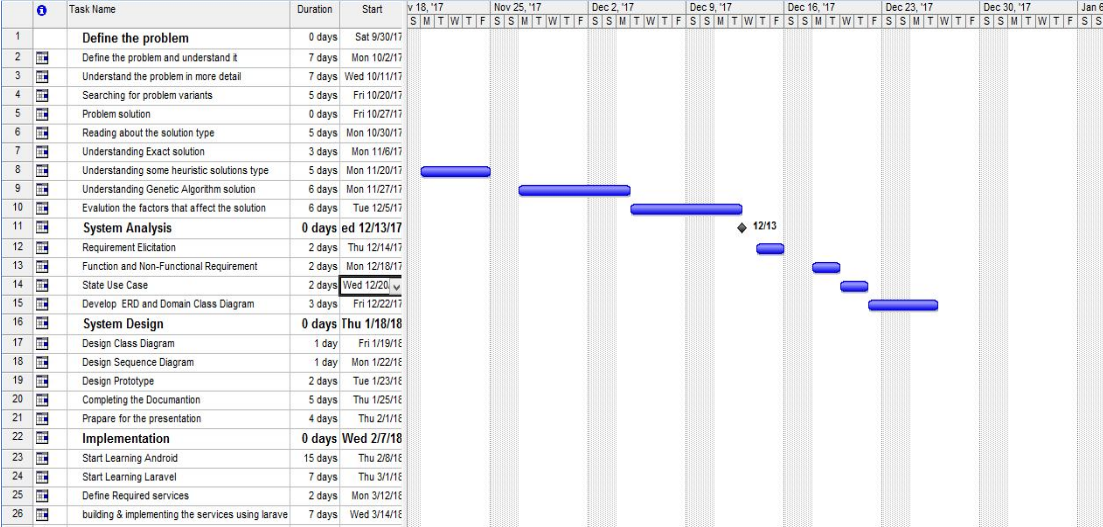
\includegraphics[width=17cm,height=8.5cm]{./assets/ganttchart/gantt-3.png}\\
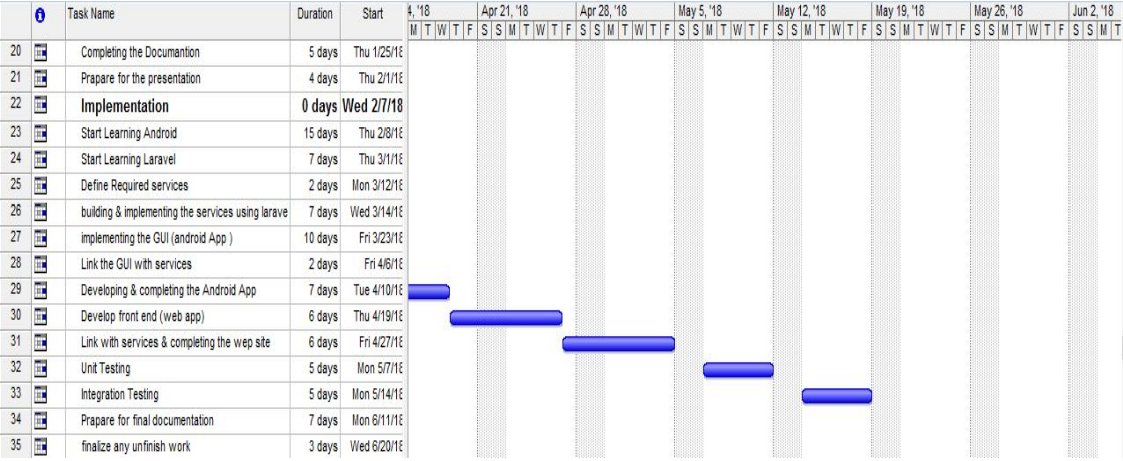
\includegraphics[width=17cm,height=8.5cm]{./assets/ganttchart/gantt-4.png}\\
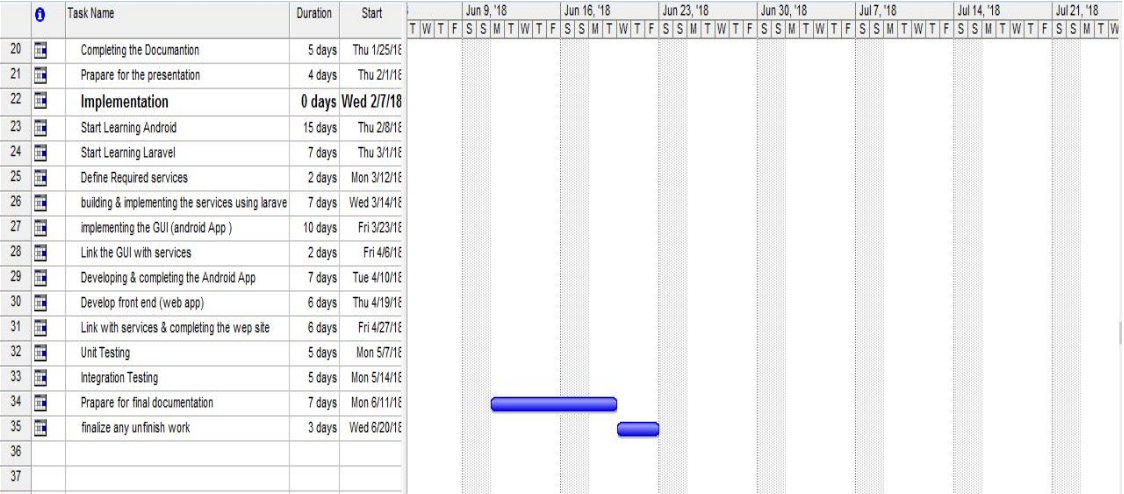
\includegraphics[width=17cm,height=8.5cm]{./assets/ganttchart/gantt-5.png}\\
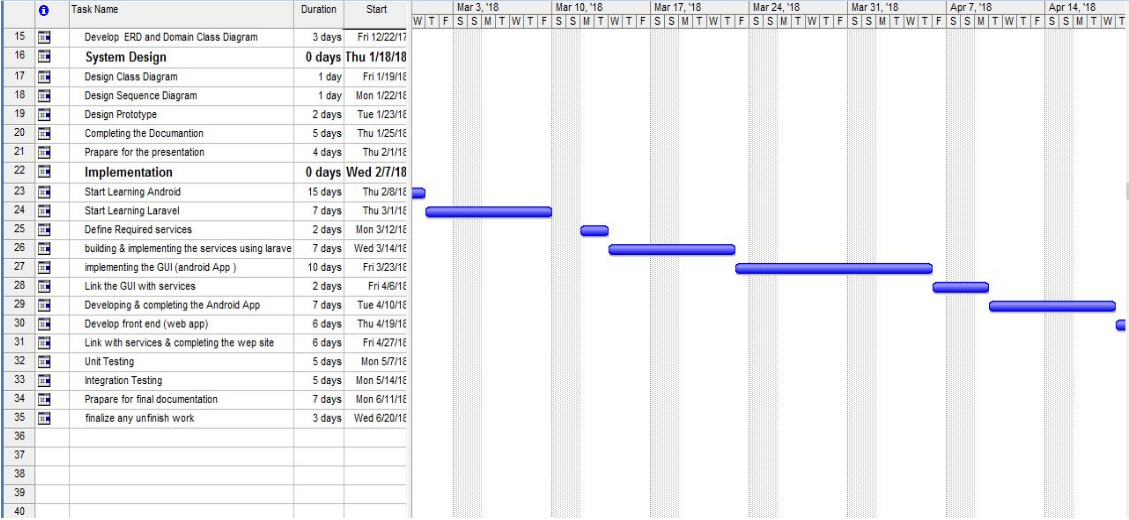
\includegraphics[width=17cm,height=8.5cm]{./assets/ganttchart/gantt-6.png}\\

\section{\sc Conclusion}
We can see now that this project will help a lot by saving money, time and efforts for the companies that have a transportation system especially the ones with large transportation systems., as the application will choose the path with the most minimum distance approximately instead of travelling longer distances, and this is done by using one of the previously mentioned. 
In this project we considered one of the factors that affect the path to choose which is the distance between different requests which is constant factor, there are other factors that taking them into consideration will make better results like traveling time, traffic, the speed limit and the types of the streets chosen whether they are highways, freeways or small streets, taking all these factors well help in making the idea more effective, but it will make the project more complex ,so we can consider them later on as a better upgrade to the project for latter versions.


\newpage

\section{\sc References}

\begin{thebibliography}{10}


\bibitem{article-minimal}
TSP.
\newblock {\href{https://en.wikipedia.org/wiki/Travelling_salesman_problem}{en.wikipedia.org/wiki/Travelling\_salesman\_problem}}

\bibitem{article-full}
TSP.
\newblock {\href{http://people.ku.edu/\~{~}jlmartin/courses/math105-F11/Lectures/chapter6-part4.pdf}{people.ku.edu/$~$lmartin/courses/math105-F11/Lectures/chapter6-part4.pdf}}

\bibitem{article-full}
Christofides Algorithm.
\newblock {\href{http://personal.vu.nl/r.a.sitters/AdvancedAlgorithms/2016/SlidesChapter2-2016.pdf}{personal.vu.nl/r.a.sitters/AdvancedAlgorithms/2016/SlidesChapter2-2016.pdf}}

\bibitem{article-full}
Christofides Algorithm.
\newblock {\href{https://en.wikipedia.org/wiki/Christofides\_algorithm}{en.wikipedia.org/wiki/Christofides\_algorithm}}

\bibitem{article-full}
Held Karp Algorithm.
\newblock {\href{https://en.wikipedia.org/wiki/Held–Karp\_algorithm}{en.wikipedia.org/wiki/Held–Karp\_algorithm}}

\bibitem{article-full}
Held Karp Algorithm.
\newblock {\href{https://www.geeksforgeeks.org/travelling-salesman-problem-set-1/}{www.geeksforgeeks.org/travelling-salesman-problem-set-1/}}

\bibitem{article-full}
Held Karp Algorithm.
\newblock {\href{https://www.youtube.com/watch?v=-JjA4BLQyqE}{www.youtube.com/watch?v=-JjA4BLQyqE}}

\bibitem{article-full}
Heuristic Algorithms.
\newblock {\href{https://web.tuke.sk/fei-cit/butka/hop/htsp.pdf}{https://web.tuke.sk/fei-cit/butka/hop/htsp.pdf}}

\end{thebibliography}


\end{document}